% Options for packages loaded elsewhere
\PassOptionsToPackage{unicode}{hyperref}
\PassOptionsToPackage{hyphens}{url}
%
\documentclass[
  openany]{book}
\usepackage{amsmath,amssymb}
\usepackage{iftex}
\ifPDFTeX
  \usepackage[T1]{fontenc}
  \usepackage[utf8]{inputenc}
  \usepackage{textcomp} % provide euro and other symbols
\else % if luatex or xetex
  \usepackage{unicode-math} % this also loads fontspec
  \defaultfontfeatures{Scale=MatchLowercase}
  \defaultfontfeatures[\rmfamily]{Ligatures=TeX,Scale=1}
\fi
\usepackage{lmodern}
\ifPDFTeX\else
  % xetex/luatex font selection
\fi
% Use upquote if available, for straight quotes in verbatim environments
\IfFileExists{upquote.sty}{\usepackage{upquote}}{}
\IfFileExists{microtype.sty}{% use microtype if available
  \usepackage[]{microtype}
  \UseMicrotypeSet[protrusion]{basicmath} % disable protrusion for tt fonts
}{}
\makeatletter
\@ifundefined{KOMAClassName}{% if non-KOMA class
  \IfFileExists{parskip.sty}{%
    \usepackage{parskip}
  }{% else
    \setlength{\parindent}{0pt}
    \setlength{\parskip}{6pt plus 2pt minus 1pt}}
}{% if KOMA class
  \KOMAoptions{parskip=half}}
\makeatother
\usepackage{xcolor}
\usepackage{longtable,booktabs,array}
\usepackage{calc} % for calculating minipage widths
% Correct order of tables after \paragraph or \subparagraph
\usepackage{etoolbox}
\makeatletter
\patchcmd\longtable{\par}{\if@noskipsec\mbox{}\fi\par}{}{}
\makeatother
% Allow footnotes in longtable head/foot
\IfFileExists{footnotehyper.sty}{\usepackage{footnotehyper}}{\usepackage{footnote}}
\makesavenoteenv{longtable}
\usepackage{graphicx}
\makeatletter
\def\maxwidth{\ifdim\Gin@nat@width>\linewidth\linewidth\else\Gin@nat@width\fi}
\def\maxheight{\ifdim\Gin@nat@height>\textheight\textheight\else\Gin@nat@height\fi}
\makeatother
% Scale images if necessary, so that they will not overflow the page
% margins by default, and it is still possible to overwrite the defaults
% using explicit options in \includegraphics[width, height, ...]{}
\setkeys{Gin}{width=\maxwidth,height=\maxheight,keepaspectratio}
% Set default figure placement to htbp
\makeatletter
\def\fps@figure{htbp}
\makeatother
\setlength{\emergencystretch}{3em} % prevent overfull lines
\providecommand{\tightlist}{%
  \setlength{\itemsep}{0pt}\setlength{\parskip}{0pt}}
\setcounter{secnumdepth}{5}
\usepackage[margin = 1in]{geometry}
\ifLuaTeX
  \usepackage{selnolig}  % disable illegal ligatures
\fi
\usepackage[]{natbib}
\bibliographystyle{apalike}
\IfFileExists{bookmark.sty}{\usepackage{bookmark}}{\usepackage{hyperref}}
\IfFileExists{xurl.sty}{\usepackage{xurl}}{} % add URL line breaks if available
\urlstyle{same}
\hypersetup{
  pdftitle={Clinical Trials 4H},
  pdfauthor={Rachel Oughton},
  hidelinks,
  pdfcreator={LaTeX via pandoc}}

\title{Clinical Trials 4H}
\author{Rachel Oughton}
\date{2023-12-18}

\usepackage{amsthm}
\newtheorem{theorem}{Theorem}[chapter]
\newtheorem{lemma}{Lemma}[chapter]
\newtheorem{corollary}{Corollary}[chapter]
\newtheorem{proposition}{Proposition}[chapter]
\newtheorem{conjecture}{Conjecture}[chapter]
\theoremstyle{definition}
\newtheorem{definition}{Definition}[chapter]
\theoremstyle{definition}
\newtheorem{example}{Example}[chapter]
\theoremstyle{definition}
\newtheorem{exercise}{Exercise}[chapter]
\theoremstyle{definition}
\newtheorem{hypothesis}{Hypothesis}[chapter]
\theoremstyle{remark}
\newtheorem*{remark}{Remark}
\newtheorem*{solution}{Solution}
\begin{document}
\maketitle

{
\setcounter{tocdepth}{1}
\tableofcontents
}
\hypertarget{welcome-to-clinical-trials-4h}{%
\chapter*{Welcome to Clinical Trials 4H!}\label{welcome-to-clinical-trials-4h}}
\addcontentsline{toc}{chapter}{Welcome to Clinical Trials 4H!}

This page contains the notes for Clinical Trials IV. As we progress through the course, more will appear. You can also download the PDF version (see the icon at the top left). If you notice any typos, mistakes or places that are unclear, please do let me know!

\hypertarget{practical-details}{%
\section*{Practical details}\label{practical-details}}
\addcontentsline{toc}{section}{Practical details}

\hypertarget{lectures}{%
\subsection*{Lectures}\label{lectures}}
\addcontentsline{toc}{subsection}{Lectures}

Our lectures are 12 noon on Mondays and 9am on Wednesdays, all in ES231. This is in the Earth Sciences / Arthur Holmes building, which is behind (almost surrounding) the Calman Learning Centre. The door of this room is actually labelled `Teaching Room 4'.

\hypertarget{computer-classes}{%
\subsection*{Computer classes}\label{computer-classes}}
\addcontentsline{toc}{subsection}{Computer classes}

We have two 2-hour practicals for this module. They are 11am - 1pm on the Fridays of weeks 14 and 19 (2nd February and 8th March). These classes are in RH-0003. This is Rowan House, which is in Upper Mountjoy, across the pond from the MCS building.

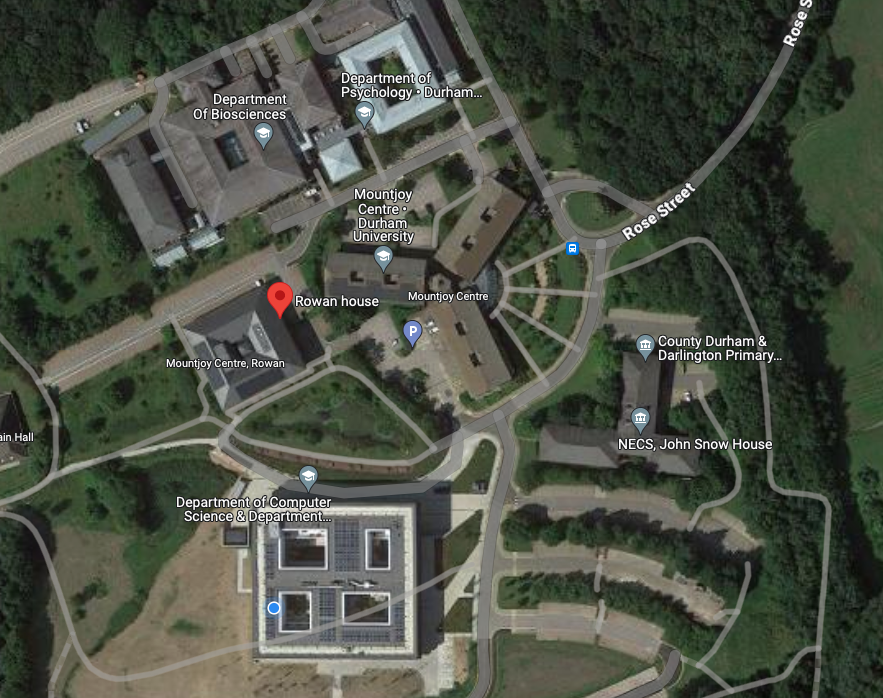
\includegraphics{images/rowanhouse_map.png}

\hypertarget{assessment}{%
\subsection*{Assessment}\label{assessment}}
\addcontentsline{toc}{subsection}{Assessment}

This module is assessed through two equally weighted pieces of coursework. The first will be assigned on Wednesday 7th February, the second on Wednesday 13th March.

There will also be some formative assignments throughout the course. More details on these to follow.

\hypertarget{books}{%
\subsection*{Books}\label{books}}
\addcontentsline{toc}{subsection}{Books}

The main reference for the first half of the course is \citet{matthews2006introduction}. There are a couple of copies in the Bill Bryson Library. Some other books we will make use of are \citet{hulley2013designing}, \citet{hayes2017cluster}. You shouldn't need to use any of these books, but of course you're welcome to if you want to read further.

\hypertarget{what-to-expect-from-this-module}{%
\section*{What to expect from this module}\label{what-to-expect-from-this-module}}
\addcontentsline{toc}{section}{What to expect from this module}

Clinical Trials IV is somewhat different from the majority of statistics modules, because

\begin{itemize}
\tightlist
\item
  It is more focussed on application than on methodology
\item
  It is assessed purely through coursework.
\end{itemize}

This means that your experience of it might be different from what you're used to

\begin{itemize}
\tightlist
\item
  We will cover quite a lot of different statistical methods (drawing on most of the 1H and 2H courses, and some 3H!) but not in great depth
\item
  There is no pressure to memorize anything - indeed, if you really were a trial statistician, you would definitely have access to the internet, various textbooks and indeed these notes (should they prove useful!).
\item
  There is an emphasis on understanding which method we use and why, and what it means. Hopefully this has been the case in some of your other modules too!
\end{itemize}

\hypertarget{what-i-expect-from-you}{%
\subsection*{What I expect from you}\label{what-i-expect-from-you}}
\addcontentsline{toc}{subsection}{What I expect from you}

Because we will be covering quite a lot of different areas within statistics, there may be some things that you haven't seen before (or can't remember very well). I will try my best to explain them as clearly as I can, but there isn't time to go into the nuts and bolts of everything we come across. Therefore, if you do feel a bit rusty on some area, you may need to read up on that a bit, so that you're happy with it. I am very happy to suggest resources from time to time, and you're welcome to come to the office hour to talk about such things.

This is the first year this course is running, and so I would also really appreciate your feedback. I may not be able to address everything (or I may only be able to implement things for following years), but if I can act on it quickly then I will!

\hypertarget{rct-intro}{%
\chapter{Introduction to Clinical Trials}\label{rct-intro}}

A clinical trial is an experiment, usually performed on human subjects, to test the effect of some sort of treatment or intervention. We may also use the term \textbf{Randomised controlled trial} (RCT). These are not fully the same thing; a clinical trial may not have been randomised, for example if it follows a pre-determined cohort through some sort of process. Likewise, an RCT may not be clinical, but instead may be about an intervention in some other setting like agriculture or education. For this module, we are really focussing on RCTs, and almost all of our examples will be clinical.

For the purposes of this module, a clinical trial will have two groups:

\begin{enumerate}
\def\labelenumi{\arabic{enumi}.}
\tightlist
\item
  The \textbf{treatment group} or \textbf{intervention group}: this group of people will be subject to the new treatment.
\item
  The \textbf{control group}: this group of people will be subject to the status quo - the `standard' or most widely used treatment path for their cohort (sometimes this is no treatment).
\end{enumerate}

These groups are usually, though not always, of the same size. Which group each patient is assigned to is usually decided by randomization, which is something we will go on to explore in later lectures. In reality, trials can have more than two groups, and many statistical methods extend quite naturally to this.

The goal of the trial is to estimate the \textbf{treatment effect}: is the treatment better than the control, and if so, how much? This short description raises lots of statistical issues, which will take up the next few weeks!

Before we get into the theory, we'll think about some of the background to clinical trials, and introduce some key ideas.

Put (very!) simply, the goal of a clinical trial is to determine what works to make people better. Although clinical trials as we know them now have only been around since the Second World War, similar sorts of experiments can be seen from much longer ago. If you're interested in learning about the evolution of clinical trials from Biblical times to now, \href{https://www.jameslindlibrary.org/}{the James Lind Library} has some fascinating resources and articles.

\begin{example}
\textbf{Scurvy (James Lind, 1757)}
Scurvy was a serious disease, particularly affecting seamen on long voyages. Symptoms were unpleasant (mouth sores, skin lesions etc.) and it could often be fatal. Lind was the ship's surgeon on board the HMS Salisbury, and had several patients with scurvy. Many remedies were proposed and in popular use at the time (with only anecdotal evidence, if any, to support them). In 1757 Lind decided to test six such treatments, on two patients each:

\begin{itemize}
\tightlist
\item
  cider
\item
  dilute sulfuric acid
\item
  vinegar
\item
  sea water
\item
  citrus (oranges and lemons)
\item
  purgative mixture (a paste of garlic, mustard seed, horseradish, balsam of Peru, and gum myrrh)
\end{itemize}

Lind chose twelve seamen with similar severity of symptoms, and subjected them to their assigned treatment for 6 days. They were kept in the same quarters, and fed the same diet apart from their treatment. Unsurprisingly (to us!) ``The most sudden and visible good effects were perceived from the use of oranges and lemons,''

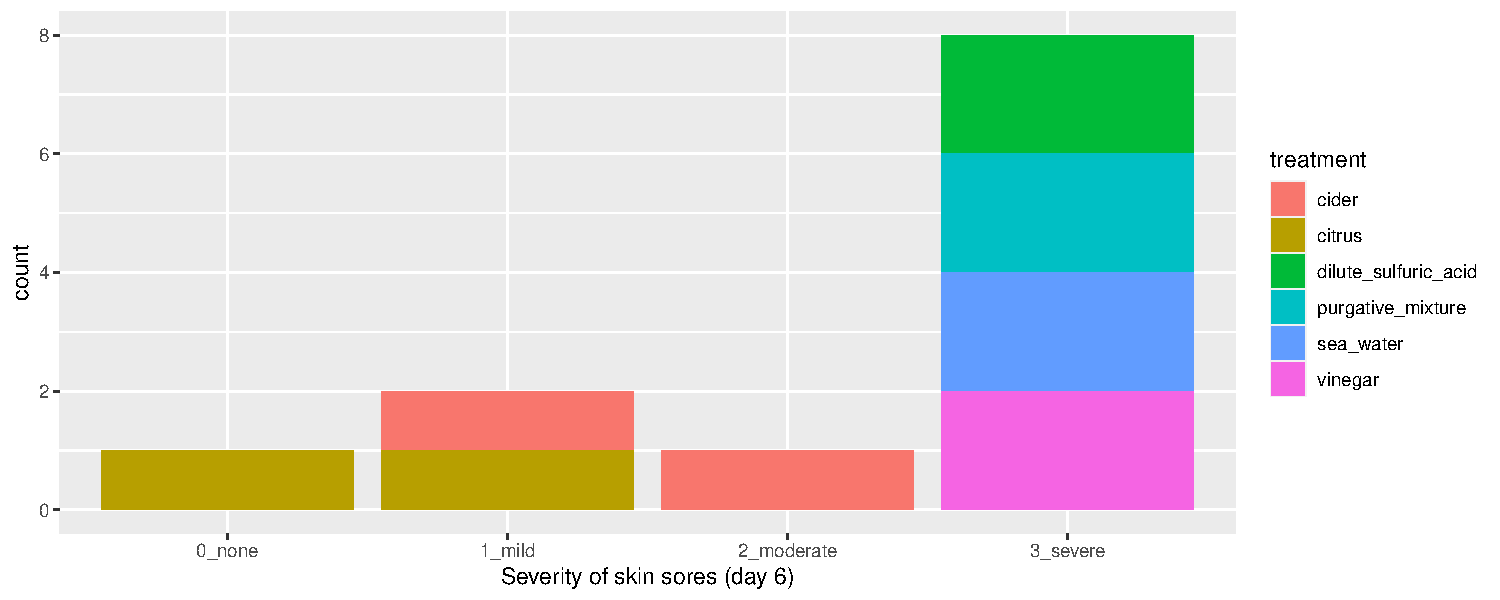
\includegraphics{CT4H_notes_files/figure-latex/unnamed-chunk-3-1.pdf}
\end{example}

A key thing to notice about the Scurvy example is that Lind went to great lengths to ensure that the treatment was the only thing affecting these 12 sailors: they all started with a similar severity of symptoms, they were kept in the same place and their diet was identical apart from their treatment. This links to one of the foundational principles of clinical trials: causal inference.

\hypertarget{causal-inference-and-clinical-trials}{%
\section{Causal inference and clinical trials}\label{causal-inference-and-clinical-trials}}

You're probably familiar with the mantra that \textbf{``correlation does not imply causation''}: just because two things are correlated, it doesn't mean we can conclude that one causes the other. If you're not convinced, \href{https://www.tylervigen.com/spurious-correlations}{here} are some humorous (and slightly macabre) examples. Causal inference is concerned with the design and analysis of data for uncovering causal relationships.

This is important for us, because we really want to be able to conclude that a treatment works (or doesn't) - that it \emph{causes} recovery, or a reduction in symptoms, or helps the patient in some way.
If we were experimental scientists in some laboratory, we could conduct some controlled experiment in which everything was kept under very specific conditions, and could fairly easily make conclusions about the treatment we were testing, and how it behaved in a range of conditions. However, testing treatments on real people is different: we don't have several identical versions of the same person to test the treatment on, and even if we did, as Gwyneth Paltrow shows us it doesn't take very much to completely alter the conditions of someone's existence!


\includegraphics{images/sliding_doors.jpeg}

Neither can we just base our conclusion of whether a treatment works on lab-based tests or theory (although undoubtedly these will both play a part in developing the treatment in the first place). The treatment needs to be tested on actual people.

Because, as we noted, people are all different, and living different lives (and unlike James Lind we can't force them all to live in the same part of a ship and eat the same food!) we will need to test the treatment on lots of people in order to gather empirical evidence. This is why statistics is so important in the design and analysis of clinical trials. The results of the trial must concluded beyond reasonable doubt, and must be able to be generalized to as-yet-untreated patients. We want to avoid any spurious correlations that are down to chance, or to associations we haven't taken into account. For example, what if the two seamen given citrus were also much younger and generally healthier than the other ten? Maybe they would have recovered quickly anyway? Or what if another treatment was actually much better than citrus, but just happened to have been given to two sailors who had some other pre-existing illness, causing them to suffer much worse with scurvy?

Clinical trials are therefore crucial for modern medicine, and statistics is crucial to clinical trials. But why exactly are clinical trials given this position of importance? Do we really have to do things this way?

\hypertarget{the-structure-of-a-clinical-trial}{%
\section{The structure of a clinical trial}\label{the-structure-of-a-clinical-trial}}

In a clinical trial, people are grouped and subdivided in various ways.

\hypertarget{the-population-of-eligible-patients}{%
\subsection*{The population of eligible patients}\label{the-population-of-eligible-patients}}
\addcontentsline{toc}{subsection}{The population of eligible patients}

One of the first steps in conducting a trial is to specify exactly what sort of person you want to test the treatment on, and where these people will be found. They may be of a certain sex and/or age range, they may have (or definitely not have) certain conditions. They may suffer from some particular symptom, or be at a particular stage of an illness.

A clear set of criteria is key to consistency. Patients are usually recruited as they present (eg. to hospital or a GP centre) and may be being recruited over several years, or by several different clinicians, so it is important that everyone is sticking to the same plan.

\begin{example}
In a study by \citet{hjalmas1998enuresis} of the use of desmopressin in children with nocturnal enuresis (bed-wetting), children had to be aged 6 - 12 with a history of PMNE (primary monosymptomatic nocturnal enuresis) and no organic pathology (no disease that alters the structure or function of organs). The children had to be free of other urinary problems (such as frequency, urgency or daytime incontinence) and not to have received any treatment for nocturnal enuresis during the 2 months before entering the trial. Children with clinically significant endocrine,
metabolic, hepatic, psychiatric, neurological, musculoskeletal, cardiovascular, haematological, renal or genitourinary disease were excluded from the trial.
\end{example}

Knowing exactly what type of patients were recruited into the trial is also key when generalizing the results to the population. If the trial recruited males aged 55-70, we cannot confidently conclude that the results will apply to a female aged 26.

\hypertarget{entry-to-the-trial}{%
\subsection*{Entry to the trial}\label{entry-to-the-trial}}
\addcontentsline{toc}{subsection}{Entry to the trial}

The group of patients recruited will be some subset of the possible population. Patients are allowed to refuse consent to take part, or individual patients may be judged unsuitable despite meeting the criteria. Knowing how many patients to recruit is a statistical question, which we will deal with soon.

\hypertarget{allocation-to-groups}{%
\subsection*{Allocation to groups}\label{allocation-to-groups}}
\addcontentsline{toc}{subsection}{Allocation to groups}

These patients are then allocated to receive either the treatment, or to be part of the control group (or more, if there are more than two groups). These groups are often referred to as the \textbf{trial arms} - the treatment arm and the control arm. Deciding which patients should be allocated to which group is another statistical question. Once the patients have been allocated, they will receive the treatment (or not) and important measurements will be taken during the trial period.

\hypertarget{comparing-results}{%
\subsection*{Comparing results}\label{comparing-results}}
\addcontentsline{toc}{subsection}{Comparing results}

Now that the trial has been run, we have two sets of measurements: one for the treatment group and one for the control group. But guess what?! Comparing these and coming to a conclusion about the effect of the treatment is a statistical question.

\hypertarget{why-bother-with-a-control-group}{%
\subsection*{Why bother with a control group?}\label{why-bother-with-a-control-group}}
\addcontentsline{toc}{subsection}{Why bother with a control group?}

Surely if we want to see whether a treatment works, we should just give it to a patient and see if they get better? Why do we need to also have a group of people not receiving the treatment?

In rare and extreme cases, this is a decent strategy: if a disease has always been fatal, but we start giving patients the treatment and some live, that is pretty solid evidence that the treatment works. This was the case with tuberculous meningitis, until the introduction of Streptomycin in 1944.

This was also the case when Edward Jenner tested cowpox as a vaccination for the fatal disease smallpox. After observing that milkmaids, once they had suffered from the mild condition cowpox (which they did often), seemed to be immune to smallpox, Jenner tested his theory by injecting an 8 year old boy called James Phipps with fluid from a milkmaid's cowpox lesions (yum). Once the boy's cowpox infection had run its course, he injected him again, this time with matter from a fresh smallpox lesion. Thankfully, James Phipps did not contract smallpox. After several more successful such tests, and a gradual shift in attitudes to the idea of vaccination (a word coined by Jenner, from the latin `vaccinia', meaning cowpox) Jenner's results were published and vaccination became commonplace. Clearly, injecting people with smallpox who had not been given the cowpox innoculation would be very cruel (they would almost certainly die) and would prove nothing; there was already plenty of evidence for the fatality of smallpox.

However, most diseases have a fairly uncertain and variable trajectory. If we give a group of patients the treatment, we can't know what would have happened to them if they hadn't received the treatment, or had received a different treatment. Comparing them to patients the past is dodgy because lots of other things may have changed since even the recent past. This is why we have a \emph{concurrent control group} (usually known as just the \emph{control group}). These patients do not receive the new treatment, but instead carry on as usual. The aim is to make the control and treatment groups as similar as possible in all other respects (especially those we deem important) so that at the end we can attribute the difference between the two groups to the treatment.

\hypertarget{primout}{%
\section{The primary outcome}\label{primout}}

In a clinical trial, there are usually many measurements performed on patients, and possibly at various different points throughout the trial. However, for the sake of the analysis, we usually determine one to be the \textbf{primary outcome variable}. The research questions should be phrased in terms of this variable, and the goal of our design should be to be able to answer questions about this variable.

\begin{example}
In a trial by \citet{villar2020dexamethasone} investigating the use of Dexamethasone treatment for acute respiratory distress syndrome , the primary outcome was the `number of ventilator free days up to 28 days', while other outcomes included `all-cause mortality after 60 days' and `incidence of infections in ICU'.
\end{example}

\hypertarget{ethical-issues}{%
\section{Ethical issues}\label{ethical-issues}}

Clinical trials differ from most scientific experiments in that they are experimenting on people. This means that the team designing, conducting and analysing the trial have various ethical responsibilities. This is a huge area; we will touch on it from time to time but will not go into anywhere near enough detail! Some key things to note though are\ldots.

\begin{itemize}
\tightlist
\item
  A patient must never be given a treatment that is known to be inferior.
\item
  Patients must be fully informed about the trial, the treatments used, possible adverse effects and side-effects and so on. Patients should only be recruited into the trial if, after being given all this information (and having had it communicated clearly and at an appropriate level) they give their consent.
\item
  After entering a trial, a patient has the right to withdraw at any point, and should then receive whatever treatment is most appropriate for them. They should not face any negative repurcussions for withdrawing.
\end{itemize}

The patients' interests are safeguarded by the \href{https://www.wma.net/policies-post/wma-declaration-of-helsinki-ethical-principles-for-medical-research-involving-human-subjects/}{Declaration of Helsinki}. This statement is implemented differently by different countries. In the UK, health authorities each have their own ethics committee, by which proposals for experiments involving human subjects must be approved.

You might think that these ethical issues largely concern the clinicians, and that we statisticians don't need to worry too much about the ethics of clinical trials. After all, we are likely never to meet any patients or to get our hands dirty in any way! But as we will see, at each stage the choices made by the statistician can in fact have serious ethical implications.

\hypertarget{phases-of-clinical-trials}{%
\section{Phases of clinical trials}\label{phases-of-clinical-trials}}

If you read about clinical trials (or hear about them in the news), you'll hear talk of a `phase 3 trial' or similar. Broadly speaking, clinical trials follow a progression from phase one (or sometimes zero) to phase four. These phases apply to most countries, and any for any drug to be licensed multinationally it must get through phase III.

\hypertarget{phase-zero}{%
\subsection*{Phase zero}\label{phase-zero}}
\addcontentsline{toc}{subsection}{Phase zero}

The first step is to test a low dose of the treatment on a small number of people, to check that it isn't harmful. The dose is too low to have any medicinal effect, but is designed to verify that the drug behaves as expected from laboratory studies, and doesn't have any harmful effects. There may only be 10-20 participants, and there is no randomisation (or control group).

\hypertarget{phase-one}{%
\subsection*{Phase one}\label{phase-one}}
\addcontentsline{toc}{subsection}{Phase one}

Phase one trials are also quite small (around 20-50 participants) and are designed to find the best dose of the treatment and what any side effects are. Phase one trials tend to be recruited very slowly: a small group will be recruited onto a low dose and monitored closely. If all goes well, another small group will be recruited on a slightly higher dose, and so on. This is known as a \emph{dose escalation study}. Participants at this phase are monitored very closely, for example through regular blood tests and recording daily symptoms.

\hypertarget{phase-two}{%
\subsection*{Phase two}\label{phase-two}}
\addcontentsline{toc}{subsection}{Phase two}

If the drug makes it through the phase one trial, it can progress to phase two (often written as `phase II'). These involve more people than phase one, possibly up to 100. The cohort may now be restricted to people with a particular version of a condition (eg. a particular type of cancer), but it may still be broader than the sorts of trials we will be looking at. Now the aim is to find out if the new treatment works well enough to progress to a large phase three (phase III) trial:

\begin{itemize}
\tightlist
\item
  Exactly what conditions (or versions of a condition) does this treatment work for?
\item
  What are the side effects and can they be managed?
\item
  What is the best dose to administer?
\end{itemize}

Phase II trials sometimes compare the treatment to a placebo, and sometimes use randomisation to group participants.

This is the stage at which most drugs fail, for a multitude of reasons (cost, safety, efficacy,\ldots).

\hypertarget{phase-three}{%
\subsection*{Phase three}\label{phase-three}}
\addcontentsline{toc}{subsection}{Phase three}

Phase III trials are much bigger, often involving hundreds or thousands of participants, and aim to compare the new treatment to the best currently available treatment (which may be another treatment, or may be nothing). Side effects are still monitored, as some of the rarer ones may not show themselves at the smaller phases, because there are fewer participants.

In phase III trials, the aim is to find out if the new treatment is better, and if so by how much. Phase III trials almost always use randomisation to allocate participants to groups, and go to great lengths to make the trial as reliable as possible, for example using a placebo for the control group (who aren't getting the real treatment) that looks identical to the real drug. These are the sorts of trials we will mainly be concerned with in this course.

To be licensed, a treatment has to get through phase III and be found to be effective (and of course safe).

\hypertarget{phase-four}{%
\subsection*{Phase four}\label{phase-four}}
\addcontentsline{toc}{subsection}{Phase four}

Phase IV trials happen after the treatment has been found to work, has been licensed and is in use. The aims of phase IV trials are

\begin{itemize}
\tightlist
\item
  to find out more about the rarer side effects
\item
  to investigate the long term risks and benefits
\item
  to find out how well the treatment works when given to a broader group of people than in phase III.
\end{itemize}

  \bibliography{ct4h.bib}

\end{document}
